
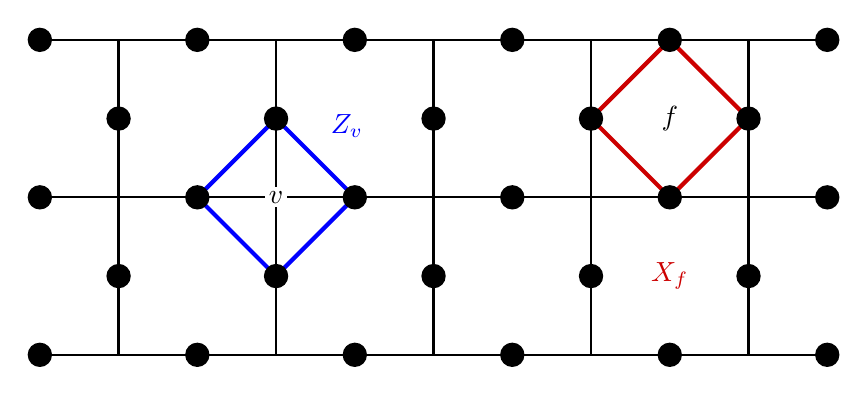
\begin{tikzpicture}[scale=2.0]

   \foreach \x in {0,1,2,3,4} {
        \draw[thick] (\x, 0) -- (\x, 2); 
    }
 
    \foreach \y in {0,1,2} {
        \draw[thick] (-0.5, \y) -- (4.5, \y);
    }

    \draw[line width=1.5pt, color=blue] 
        (1, 0.5) -- (1.5, 1) -- (1, 1.5) -- (0.5, 1) -- cycle;

    \node[fill=white, inner sep=1.5pt, text=black] at (1,1) {$v$};


    \node[text=blue] at (1.45, 1.45) {$Z_v$};

    \draw[line width=1.5pt, color=red!80!black] 
        (3.5, 1) -- (4, 1.5) -- (3.5, 2) -- (3, 1.5) -- cycle;

    \node[text=black] at (3.5, 1.5) {$f$};
    \node[text=red!80!black] at (3.5, 0.5) {$X_f$};

    \foreach \y in {0,1,2} {
        \foreach \x in {-0.5, 0.5, 1.5, 2.5, 3.5, 4.5} {
            \fill[black] (\x, \y) circle (2.2pt);
        }
    }
    \foreach \x in {0,1,2,3,4} {
        \foreach \y in {0.5, 1.5} {
            \fill[black] (\x, \y) circle (2.2pt);
        }
    }

\end{tikzpicture}